\documentclass{article}
\usepackage[utf8]{inputenc}
\usepackage{amsfonts}
\usepackage{amsmath}
\usepackage{amsthm}
\usepackage{etoolbox}
\usepackage{dynkin-diagrams}
\usepackage{float}
\usepackage[english]{babel}
\usepackage{enumitem}

\newtheorem{theorem}{Theorem}
\newtheorem{corollary}{Corollary}[theorem]
\newtheorem{lemma}[theorem]{Lemma}
\theoremstyle{definition}
\newtheorem{definition}{Definition}[section]

\tikzset{
    /Dynkin diagram,
        indefinite edge/.style={
            thick,
            dashed
        },
        o/.style={
            thick,
            fill=white,
            draw=black
        },
        edge length=1.5cm, 
        edge/.style={thick}, 
        arrow style={black,
                length=3mm,
                width=5mm,
                line width=1pt
                },
        root radius=.15cm,
        mark=o}

\title{Classification of Semisimple Lie Algebras via Root Systems using Dynkin Diagrams}
\author{Young He}
\date{June 2022}

\begin{document}

\maketitle

\section*{Abstract}
\quad The Euclidean space, when viewed solely by itself as a vector space, often comprise of little information or structure of interest. However by studying the properties of finite collections of its vectors under specific conditions, we can produce structures that are interesting algebraically. In particular, root systems are finite spanning sets of vectors (known as ``roots") in the Euclidean space that satisfy a list of special properties. Moreover, root systems show up naturally in the study of Lie theory; in particular, it turns out that all semisimple Lie algebras can be identified by an associated root system. The structure of root systems are quite simple; in fact, the complete classification of (irreducible) root systems can be stated in a straightforward manner. \\

Although root systems are quite algebraic in nature, they can be studied even more thoroughly under a combinatorial framework. Tools such as the Dynkin diagram help establish important connections between the algebraic and combinatoric aspects of root systems, by providing a direct correspondence of root systems and simpler graph theoretic structures. This construct is central to the classification of irreducible root systems, and allows such classifications to be stated in a succinct manner. These classifications can then be used to completely classify simple Lie algebras, and are even applicable to the larger class of semisimple Lie algebras. 

\section*{Reference Materials}
\begin{itemize}
    \item \textit{Lie Groups, Lie Algebras, and Representations} (B. Hall)
    \item \textit{Introduction to Lie Algebras and Representation Theory} (J. Humphreys)
\end{itemize}

\newpage

\section{Introduction to Root Systems}
\quad Let $E$ be a finite-dimensional (real) vector space with inner product $\langle\cdot,\cdot\rangle$. We axiomatically define a \textbf{root system} to be a finite set $R$ of nonzero vectors in $E$, such that the following properties are satisfied for any $\alpha,\beta\in R$: 
\begin{enumerate}
    \item $\mbox{span}(R)=E$
    \item $c\alpha\in R\implies c=\pm1$
    \item $s_\alpha(\beta)\in R$, where $s_\alpha(\beta)=\beta-2\frac{\langle\alpha,\beta\rangle}{\langle\alpha,\alpha\rangle}\alpha$
    \item $2\frac{\langle\alpha,\beta\rangle}{\langle\alpha,\alpha\rangle}\in\mathbb{Z}$
\end{enumerate}
\quad Moreover, we refer to the dimension of $E$ as the \textbf{rank} of $R$, and elements in $R$ are called \textbf{roots}. Notably, all of the above properties have quite intuitive geometric meanings. For example, consider $(3)$: as a basic linear algebra result, $s_\alpha(\beta)$ reflects $\beta$ across the hyperplane orthogonal to $\alpha$. Thus, $(3)$ requires root systems to be closed under such reflections; and conditions $(1)$, $(2)$, and $(4)$ likewise impose other restrictions on the structural closure of root systems. \\

In fact, the four axioms are extremely restrictive. We now prove that both the angular and length-wise relations between two roots only have a fixed set of possibilities: 
\begin{theorem}
Let $\alpha,\beta$ be two roots in the root system $R$ (let $|\alpha|\geq|\beta|$), and denote the angle between them as $\theta$. Then, one of the following must be true: 
\begin{enumerate}
    \item $\langle\alpha,\beta\rangle=0$ (i.e. they are perpendicular)
    \item $\langle\alpha,\alpha\rangle=\langle\beta,\beta\rangle$, with $\theta=\frac{\pi}{3},\frac{2\pi}{3}$
    \item $\langle\alpha,\alpha\rangle=2\langle\beta,\beta\rangle$, with $\theta=\frac{\pi}{4},\frac{3\pi}{4}$
    \item $\langle\alpha,\alpha\rangle=3\langle\beta,\beta\rangle$, with $\theta=\frac{\pi}{6},\frac{5\pi}{6}$
\end{enumerate}
\end{theorem}
\begin{proof}
We will show that if (1) is not true, then one of (2), (3), or (4) must be. Let $m_1=2\frac{\langle\alpha,\beta\rangle}{\langle\alpha,\alpha\rangle}$ and $m_2=2\frac{\langle\beta, \alpha\rangle}{\langle\beta,\beta\rangle}$: it is clear from definitions that $m_1,m_2\in\mathbb{Z}$. Now, note that: 
$$m_1 m_2=4\frac{\langle\alpha,\beta\rangle^2}{\langle\alpha,\alpha\rangle\langle\beta,\beta\rangle}=4\cos^2\theta$$
And since we assumed $\langle\alpha,\beta\rangle\neq0$, we have $0<m_1m_2\leq4$. Also since $\alpha$ and $\beta$ must be linearly independent, $\cos\theta\neq1$ so $m_1m_2$ can only be 1, 2, or 3. 
\begin{enumerate}
    \item If $m_1m_2=1$, then $\theta=\cos^{-1}(\frac{1}{2})=\frac{\pi}{3},\frac{2\pi}{3}$. Since both $m_1$, $m_2$ are integers, $m_1=m_2=\pm1$. Then, $\langle\alpha,\alpha\rangle=\pm2\langle\alpha,\beta\rangle=\langle\beta,\beta\rangle$ i.e. we have case (2). 
    \item If $m_1m_2=2$, then $\theta=\cos^{-1}(\frac{\sqrt{2}}{2})=\frac{\pi}{4},\frac{3\pi}{4}$. Since $|\alpha|\geq|\beta|$, we must have $m_1=1,m_2=2$ or $m_1=-1,m_2=-2$. But in either case,  $\langle\alpha,\alpha\rangle=\pm2\langle\alpha,\beta\rangle=2\langle\beta,\beta\rangle$ i.e. we have case (3). 
    \item If $m_1m_2=3$, then $\theta=\cos^{-1}(\frac{\sqrt{3}}{2})=\frac{\pi}{6},\frac{5\pi}{6}$. Similar to the last scenario, we must have $m_1=\pm1,m_2=\pm3$. This yields $\langle\alpha,\alpha\rangle=\pm2\langle\alpha,\beta\rangle=3\langle\beta,\beta\rangle$, i.e. we have case (4). 
\end{enumerate}
So either one of (1), (2), (3), or (4) must hold, as desired. 
\end{proof}
Furthermore, each of these four cases corresponds to a distinct rank 2 root system; in fact, they actually describe the complete classification of rank 2 root systems. But first, we need define the isomorphism between root systems: two root systems $R$ (over $E$), $S$ (over $F$) are considered \textbf{isomorphic} if there exists an invertible $\varphi : E\to F$, such that $\varphi\circ s_\alpha=s_{\varphi(\alpha)}\circ\varphi$ for every $\alpha\in R$. In other words, all reflections $s_\alpha$ are preserved under $\varphi$. 
\begin{corollary}
The four root systems in the figure below (demonstrated over $\mathbb{R}^2$) are the only rank 2 root systems, up to isomorphism. 
\end{corollary}
\begin{figure}[H]
  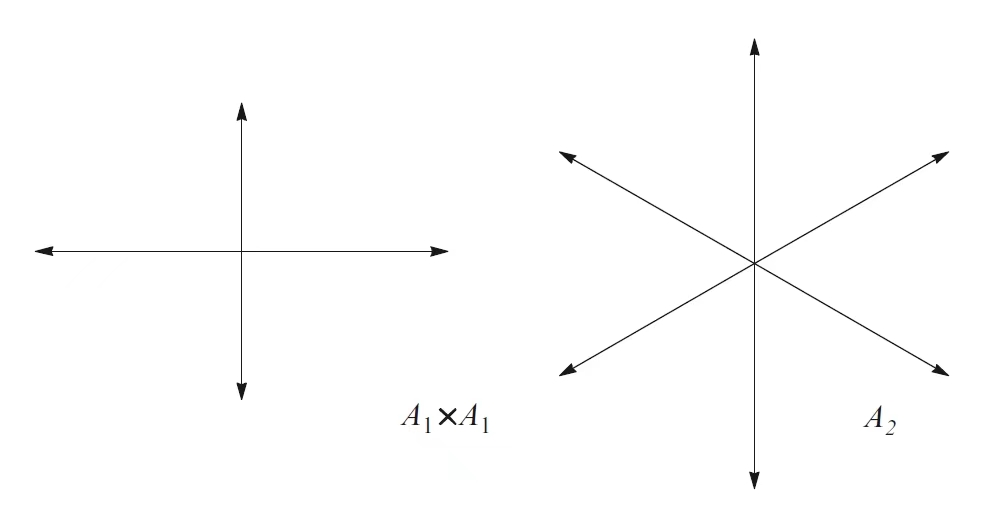
\includegraphics[width=0.5\textwidth]{top.jpg}
  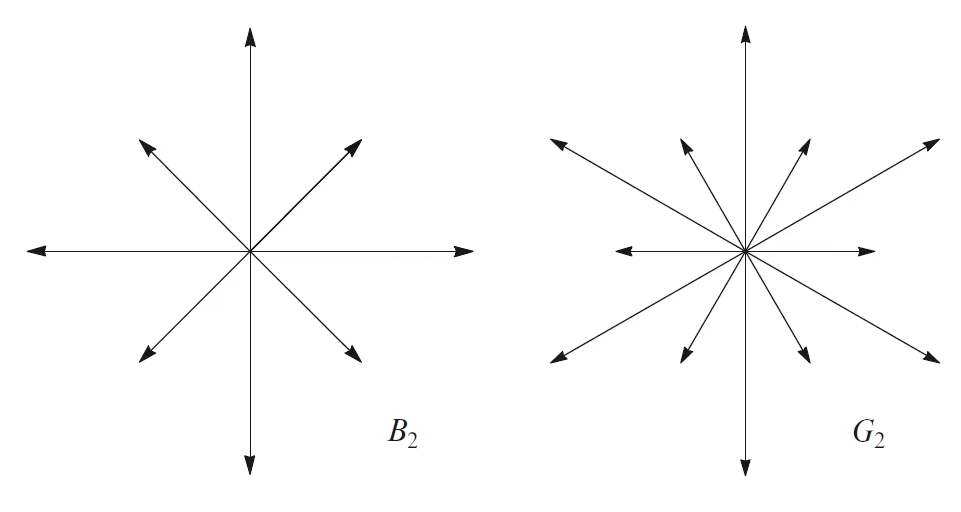
\includegraphics[width=0.5\textwidth]{bottom.jpg}
  \caption{Root systems of rank 2 (Credit: B. Hall)}
\end{figure}
This is a simple (yet insightful) illustration of how root systems can be classified elegantly. Later in this text, we shall examine the complete classification of root systems with arbitrary ranks. 
\section{Bases and Weyl Groups}
\quad Now that we have a basic understanding of how root systems work, we can introduce some important concepts about them. In particular, we wish to characterize root systems using the least amount of information possible. Similar to how we can study a vector space using its basis, we want to determine a minimal subset of a root system $R$ that still retains all the relevant information. The following construct achieves this exact purpose: a subset $\Delta$ is a \textbf{base} of $R$ if $\Delta$ is a basis of the underlying vector space $E$, and that for every $\alpha\in R$, $\alpha=\sum_{\delta\in\Delta}k_\delta\delta$ such that each $k_\delta$ has the same sign (i.e. all non-negative or non-positive). We call elements of $\Delta$ \textbf{simple roots}. A few important properties of $\Delta$ are obvious: 
\begin{enumerate}
    \item $\Delta$ has cardinality $\dim(E)$
    \item Each $\alpha\in R$ can be \textit{uniquely} decomposed in terms of $\Delta$
    \item The decompositions in (2) have integer coefficients
\end{enumerate}
\quad It is important to note that bases always exist for any given root system. However, the proof for this statement is very convoluted and thus omitted for concision (interestingly, the proof is actually constructive). But although bases exists for every root system, it is never unique: the trivial rank 1 root system serves as a simple example (both $\{1\}$ and $\{-1\}$ are valid bases). To address this, we show that all bases are indeed equivalent under a specific relation. We define the \textbf{Weyl group} $W$ of a root system $R$ (over $E$) to be the subgroup of $O(E)$, the orthogonal group over $E$, that is generated by the reflections $s_\alpha$. \\

The following theorem, given without proof, demonstrates that different bases of the same root system are equivalent under actions of $W$: 
\begin{theorem}
The group $W$ acts transitively over $R$. Furthermore, for any bases $\Delta_1$ and $\Delta_2$ of $R$, there exists $w\in W$ such that $w:\Delta_1\mapsto\Delta_2$. 
\end{theorem}
The implications of this theorem is quite similar to how different sets of basis vectors can represent the same vector space, but they can all be related to one another via a change of basis matrix. From this, we see that all bases of a root system are equivalent to some degree; indicating that they can be used to represent root systems in a more succinct manner. 
\section{Dynkin Diagrams}
\quad As we see from before, bases convey the most essential information about root systems using minimal elements. Now, recall Theorem 1: we deduced that the angular and length-wise relation between two roots have limited possibilities. And since the base $\Delta$ is finite, we can represent the relations between the simple roots by using a graph-like structure. A \textbf{Dynkin diagram} is a graph with elements in $\Delta$ as vertices, where the type of edge between $\alpha,\beta\in\Delta$ is identified by:  
\begin{enumerate}
    \item if $\langle\alpha,\beta\rangle=0$, we don't draw an edge between $\alpha$ and $\beta$. 
        $$\beta \quad \dynkin A1 \quad \quad \quad \dynkin A1 \quad \alpha$$
    \item if $\frac{|\alpha|^2}{|\beta|^2}=1$, we draw a single edge between $\alpha$ and $\beta$. 
    $$\beta \quad \dynkin A2 \quad \alpha$$
    \item if $\frac{|\alpha|^2}{|\beta|^2}=2$, we draw a double edge between $\alpha$ and $\beta$, with an arrow from $\beta$ to $\alpha$. 
    $$\beta \quad \dynkin B2 \quad \alpha$$
    \item if $\frac{|\alpha|^2}{|\beta|^2}=3$, we draw a triple edge between $\alpha$ and $\beta$, with an arrow from $\beta$ to $\alpha$. 
    $$\beta \quad \dynkin G2 \quad \alpha$$
\end{enumerate}
This allows us to visualize a root system in a graphical manner. We can also define an \textbf{isomorphism} between Dynkin diagrams to be a map that preserves the vertices and edge types (including directions). This is neat; however, the structure of \textit{any} Dynkin diagram can be arbitrary due to the possibility of disconnected graphs. And because we are aiming to \textit{classify} root systems, it would be more helpful to limit our scope to the Dynkin diagrams that are \textbf{connected}. In this regard, we introduce another useful definition: a root system $R$ over $E$ is called \textbf{reducible} if $E=E_1\oplus E_2$ such that $R$ falls entirely in $E_1$ or $E_2$. The following theorem demonstrates the correspondence between root systems and Dynkin diagrams: 

\begin{theorem}
A root system is irreducible if and only if its Dynkin diagram is connected. Moreover, root systems are isomorphic if their Dynkin diagrams are. 
\end{theorem}
\begin{proof}
We will only prove the first statement for the sake of concision. 

$(\implies)$ Let the root system $R$ over $E$ be reducible, such that $E=E_1\oplus E_2$ and $R$ decompose into the $R_1\subset E_1, R_2\subset E_2$. We would also be able to decompose $\Delta=\Delta_1\cup\Delta_2$: where $\Delta_1$ and $\Delta_2$ are bases for $R_1$ and $R_2$ respectively. Since $R_1$ and $R_2$ are in orthogonal subspaces, each pair of simple roots between $\Delta_1$ and $\Delta_2$ are orthogonal, i.e. $\Delta_1$, $\Delta_2$ are disconnected on the Dynkin diagram of $\Delta$. 

$(\impliedby)$ Let the Dynkin diagram of $R$ be disconnected. Then, identify the two subsets $\Delta_1\cup\Delta_2=\Delta$ that are represented by disconnected subgraphs in the Dynkin diagram. If we now let $E_1=\mbox{span}(\Delta_1)$ and $E_2=\mbox{span}(\Delta_1)$, then by definition, $E=E_1 \oplus E_2$. If we let $R_1$ and $R_2$ be the subset of $R$ inside $E_1$ and $E_2$ respectively, one can easily verify that they are root systems with bases $\Delta_1$ and $\Delta_2$. 

Now, we have to show that $R_1$ and $R_2$ cover $R$ completely. Consider an arbitrary $\beta\in\Delta_1$: the reflection $s_\beta$ will be invariant on $\Delta_2$ since $\beta$ is orthogonal to all of $E_2$; likewise, $s_{\gamma}$ for any $\gamma\in\Delta_2$ will not affect $\Delta_1$. By definition, the Weyl group $W$ of $R$ is generated by all the $s_\alpha$'s ($\alpha\in R$); but since the reflection defined by elements from $\Delta_1$ and $\Delta_2$ do not affect the other set, we can write each $s_\alpha$ as some $s_\beta s_\gamma$. But by definition, the Weyl groups $W_1,W_2$ for $R_1,R_2$ are generated by $s_\beta$'s and $s_\gamma$'s respectively; i.e. $W=W_1\times W_2$. Furthermore, $W\cdot\Delta= R$ must hold as a consequence of Theorem 2; so: 
$$R=W\cdot \Delta = (W_1\times W_2)\cdot (\Delta_1 \cup \Delta_2)=(W_1\cdot\Delta_1)\cup(W_2\cdot\Delta_2)=R_1\cup R_2$$

Thus showing that $R$ is reducible to $R_1$ and $R_2$. 
\end{proof}
For example, the root system $A_1\times A_1$ (as shown in Figure 1) has a Dynkin diagram of two disjoint points; thus, the theorem above indicates that it is reducible. The implications of this theorems are deep: basically, we learned that relations between Dynkin diagrams correspond almost perfectly to relations between their underlying root systems. This indicates that root systems can be categorized just by looking at their Dynkin diagrams, thus converting the classification problem from a (complicated) algebraic one into a (relatively simple) combinatorical one. 

\section{Semisimple Lie Algebras}
\quad But before we dive into the complete classification of root systems, it would be helpful for us to connect root systems to Lie theory. In particular, root systems arise naturally when examining the properties of some special Lie algebras. A Lie algebra $\mathfrak{g}$ is called \textbf{reductive} if $\mbox{Rad}(\mathfrak{g})=Z(\mathfrak{g})$; furthermore, we call $\mathfrak{g}$ \textbf{semisimple} if it is both reductive and have a trivial center $Z(\mathfrak{g})$. One might wonder why the name \textit{semisimple} is used to describe such Lie algebras; the following theorem hopefully clarifies on the naming. 

\begin{theorem}
A semisimple Lie algebra $\mathfrak{g}$ can be decomposed uniquely as $\mathfrak{g}=\bigoplus\mathfrak{g}_i$, where each $\mathfrak{g}_i$ is a \textit{simple} Lie algebra. 
\end{theorem}

But so far, nothing obvious shows that semisimple Lie algebras have anything to do with root systems. We now introduce a substructure of semisimple Lie algebras that can be intuitively studied with the methods of root systems. A \textbf{Cartan subalgebra} $\mathfrak{h}$ of $\mathfrak{g}$ is a nilpotent subalgebra that self-normalizes, i.e. $N_\mathfrak{g}(\mathfrak{h})=\{X\in\mathfrak{g}\mid[X,H]\in\mathfrak{h},\forall H\in\mathfrak{h}\}=\mathfrak{h}$. Similar to bases for root systems, the following theorem establishes the existence and (somewhat) uniqueness of Cartan subalgebras: 
\begin{theorem}
The following are true for a (complex) semisimple Lie algebra $\mathfrak{g}$: 
\begin{enumerate}
    \item A Cartan subalgebra exists in $\mathfrak{g}$. In particular, any maximal commutative subalgebra of $\mathfrak{g}$ contains a Cartan subalgebra. 
    \item Cartan subalgebras are conjugate by elements of the associated Lie group. 
\end{enumerate}
\end{theorem}
In other words, Cartan subalgebras characterize semisimple Lie algebra almost completely. More importantly, we have the following fact about Cartan subalgebras: 
\begin{theorem}
Let $\mathfrak{h}$ be a Cartan subalgebra of a semisimple Lie algbera $\mathfrak{g}$, and let $R$ be the collection of elements $\alpha\in\mathfrak{h}$ that satisfies $[H,X]=\langle\alpha,H\rangle X$. Then, $R$ forms a root system when viewing it from the underlying inner product space. 
\end{theorem}
Finally, we see how root systems are innately rooted in Lie theory (haha, get it?). But even \textit{this} isn't where the connection between semisimple Lie algebras and root systems ends; more interestingly: 
\begin{theorem}
A semisimple Lie algebra is simple if and only if the underlying root system of its Cartan subalgebras has a connected Dynkin diagram. 
\end{theorem}
According to this theorem, the simplicity of a semisimple Lie algebra is completely determined by its Cartan subalgebras, which are characterized by their associated root systems, which then corresponds to their Dynkin diagrams. This, together with the earlier Theorem 5, indicates that we can study semisimple Lie algebras completely in terms of the associated Dynkin diagrams of its decomposition into simple components (see Theorem 4). 

\section{Classical Root Systems}
\quad Now, we examine the corresponding root systems of some simple Lie algebras. In particular, we will focus on four categories, known as the \textbf{classical Lie algebras}: $\mathfrak{sl}(n+1,\mathbb{C})$, $\mathfrak{so}(2n,\mathbb{C})$, $\mathfrak{so}(2n+1,\mathbb{C})$, and $\mathfrak{sp}(n,\mathbb{C})$. Since the underlying vector spaces of these Lie algebras are all Euclidean spaces, we let $\{e_i\}$ denote the standard basis. 
\subsection{$\mathfrak{sl}(n+1,\mathbb{C})$}
\quad The special linear Lie algebras have an underlying $E$ as the subspace of $\mathbb{R}^{n+1}$ that only contains vectors with zero-sum entries, i.e.
$$E=\{x=(x_1,\dots,x_{n+1})\mid\sum x_i=0, x\in\mathbb{R}^{n+1}\}$$

Its roots are of the form $e_j - e_k$ where $j\neq k$, so we can take $\Delta=\{e_j-e_{j+1}\}$ to be a valid base. It is clear that all simple roots are of the same length, and consecutive pairs of bases have angle $\frac{2\pi}{3}$ in between (otherwise orthogonal). The Dynkin diagram will look like: 
$$\dynkin A{}$$

We denote this category of root systems as $A_n$. 
\subsection{$\mathfrak{so}(2n,\mathbb{C})$}
\quad The special orthogonal Lie algebras have an underlying vector space of $E=\mathbb{R}^n$. When the dimension is even, its roots are of the form $\pm e_j \pm e_k$ where $j\neq k$. We can let $\Delta$ be the collection of all $\{e_j-e_{j+1}\}$'s, together with  an additional $e_{n-1}+e_n$. It is still clear that all of the members in the basis have the same length, similar to the case of $A_n$. However, $e_{n-1}+e_n$ is orthogonal to all other simple roots, but makes an angle of $\frac{2\pi}{3}$ with $e_{n-2}-e_{n-1}$. This means that the Dynkin diagram will have a ``Y" shaped branch at the end (contrary to the completely linear $A_n$). The Dynkin diagram will look like: 
$$\dynkin D{}$$

We denote this category of root systems as $D_n$. 
\subsection{$\mathfrak{so}(2n+1,\mathbb{C})$}
\quad Similar to the previous case, $E=\mathbb{R}^n$. However, we now consider the case when the dimension of the special orthogonal Lie algebra is odd. In this case, we can admit more roots: in addition to the usual $\pm e_j \pm e_k$ ($j\neq k$), vectors of the form $\pm e_j$ are also roots. To build a base for odd special orthogonal Lie algebras, we start $\Delta$ with the same list of $\{e_j-e_{j+1}\}$'s; however, we append a $e_n$ instead of the $e_{n-1}+e_n$ in the previous case. This is clearly a minimally spanning set of roots, so $\Delta$ is a base. Via some simple manipulations, one can verify that all non-consecutive entries in $\Delta$ are orthogonal, and consecutive entries other than $e_n$ have angular relations of $\frac{2\pi}{3}$. Furthermore, $e_n$ and $e_{n-1}-e_n$ makes an angle of $\frac{3\pi}{4}$. The Dynkin diagram will look like: 
$$\dynkin B{}$$

We denote this category of root systems as $B_n$. Note that $|e_n|<|e_{n-1}-e_n|$, so the arrow on the last double-edge points to the right. 
\subsection{$\mathfrak{sp}(n,\mathbb{C})$}
\quad The symplectic Lie algebras also have $E=\mathbb{R}^n$. The roots are quite similar to the previous case: in addition to $\pm e_j \pm e_k$ ($j\neq k$), vectors of the form $\pm2e_j$ (contrary to the $\pm e_j$ from before) are also allowed. To build a base $\Delta$, we still start with the usual list of $\{e_j-e_{j+1}\}$'s; however, we use $2e_n$ for the last ``special root". The angular relations between the simple roots are the same as the previous case; however, $|2e_n|>|e_{n-1}-e_n|$ so the length-wise relation between the last two nodes are reversed. The Dynkin diagram will look like: 
$$\dynkin C{}$$

We denote this category of root systems as $C_n$. Note that this is almost the same as the previous case, other than the arrow on the last double-edge pointing to the left. \\

These four categories of simple Lie algebras are special: it turns out, they are the \textit{only} infinite families of simple Lie algebras to exist (up to isomorphism), and this is exactly the rationale behind the name ``classical" Lie algebras. 

\section{Classification of Root Systems}
Finally, we are ready to present the most important result from this text. It turns out that \textit{most} Dynkin diagrams fall into one of the categories listed in the previous section; however, there are a few exceptions. We will list the exceptions below, but their corresponding root systems (thus, related Lie algebras) will not be presented. The \textbf{exceptional Dynkin diagrams}, corresponding to the \textbf{exceptional root systems}, are: 
\begin{itemize}
    \item $E_6$: $\dynkin E6$
    \item $E_7$: $\dynkin E7$
    \item $E_8$: $\dynkin E8$\\
    \item $F_4$: $\dynkin F4$\\
    \item $G_2$: $\dynkin G2$ (note: we've seen this guy before, it has rank 2)
\end{itemize}
And now, we can state the complete classification of (irreducible) root systems: 
\begin{theorem}
Every irreducible root system is isomorphic to, one and exactly one of the following:
\begin{itemize}
    \item The classical root systems: $A_n$ $(n\geq1)$, $B_n$ $(n\geq2)$, $C_n$ $(n\geq3)$, $D_n$ $(n\geq4)$
    \item The exceptional root systems: $E_6$, $E_7$, $E_8$, $F_4$, $G_2$
\end{itemize}
\end{theorem}
Observe the limiting indices for the classical root systems: they are in place to prevent double counting (e.g., $A_3\cong D_3$) and to exclude reducible ones from being listed (e.g., $D_2$). More importantly, as we have mentioned before, the classification of root systems directly corresponds to simple Lie algebras: 
\begin{corollary}
Every (complex) simple Lie algebra is isomorphic to, one and exactly one of the following:
\begin{itemize}
    \item The classical Lie algebras: $\mathfrak{sl}(n+1,\mathbb{C})$, $\mathfrak{so}(2n,\mathbb{C})$, $\mathfrak{so}(2n+1,\mathbb{C})$, $\mathfrak{sp}(n,\mathbb{C})$
    \item The exceptional Lie algebras: $\mathfrak{e}_6$, $\mathfrak{e}_7$, $\mathfrak{e}_8$, $\mathfrak{f}_4$, $\mathfrak{g}_2$
\end{itemize}
\end{corollary}
From here, we can use the unique decomposition of any semisimple Lie algebra $\mathfrak{g}$ into simple Lie algebras $\mathfrak{g}_i$ (according to Theorem 4), and count the occurrence of each classical / exceptional Dynkin diagram from the $\mathfrak{g}_i$'s. This information completely determines the structure of $\mathfrak{g}$ up to isomorphism, so our classification of semisimple Lie algebras is complete. 

\section{Concluding Remarks}
\quad The classification of root systems, and therefore the classification of all semisimple Lie algebras, is often regarded to as one of the most elegant results in Lie theory. It is often compared to the complete classification of finite simple groups; however, the proof for that result is vastly more complicated -- and even the statement itself is much more involved. \\

Lie theory has far reaching effects in many different areas of mathematics; and the classification results, such as the one presented here, can be generalized to give more insight into many different algebraic structures. Moreover, Lie algebras arise naturally in other subjects of scientific study: physics, computer science, etc. This further ascertains the importance of the study of different Lie algebras, and shows that Lie theory has an overarching importance across many different subjects -- not just within Mathematics. 

\end{document}
